% Created 2022-12-01 Thu 12:09
% Intended LaTeX compiler: pdflatex
\documentclass[11pt,a4paper]{article}
    \usepackage[utf8]{inputenc}
    \usepackage[T1]{fontenc}
    \usepackage{fixltx2e}
    \usepackage{graphicx}
    \usepackage{longtable}
    \usepackage{float}
    \usepackage{wrapfig}
    \usepackage{rotating}
    \usepackage[normalem]{ulem}
    \usepackage{amsmath}
    \usepackage{textcomp}
    \usepackage{marvosym}
    \usepackage{wasysym}
    \usepackage{amssymb}
    \usepackage{hyperref}
    \usepackage{mathpazo}
    \usepackage{color}
    \usepackage{enumerate}
    \definecolor{bg}{rgb}{0.95,0.95,0.95}
    \tolerance=1000
                    \usepackage{listings}
\usepackage{xcolor}
\lstset{language=Python,backgroundcolor=\color{black!5}, basicstyle=\footnotesize\ttfamily, columns=fullflexible, breaklines, frame= tb}

    \linespread{1.1}
    \hypersetup{pdfborder=0 0 0}
\author{Ved Patel 67 Vijay Panchal 68}
\date{\today}
\title{Timebomb of approximation in physics}
\hypersetup{
 pdfauthor={Ved Patel 67 Vijay Panchal 68},
 pdftitle={Timebomb of approximation in physics},
 pdfkeywords={},
 pdfsubject={},
 pdfcreator={Emacs 28.1 (Org mode 9.5.2)}, 
 pdflang={English}}
\begin{document}

\maketitle
\tableofcontents

\pagebreak
\section{Introduction}
\label{sec:org5ac4def}

Approximation method is yet most essential topic in physics. Also, approximation is yet essential trick for physicists. Physicists love to do approximations, like in functional expansion for getting polynomials for their ease or may be specialized idealization in particular topic. Approximation help them to \textbf{seeing through physics} instead of going in to maze of exactness in formidable  mathematics. Getting interpretation or i say knowing system is sometime more important then going for regorious mathematics. For example, famous equation of fluid dynamics \textbf{Navier-Stoke equation} can be imposible to solve but as physicist they know what it is.

Be aware, that approximation is just approximation. We should remember everytime we do that. Sometime we forgot actual system which is far from ideal. We should know that we are on mission to know nature not just building new theories.

Let's dive into one example, that showes implication of approximations. In classical mechanics, we have some major theories, one is of oscillatory motions. In Oscillation theory we studied \textbf{Simple Harmonic Oscillation}, but as we are going to see that simple harmonic oscillation is not exactly that simple without approximation. We had actually changed whole system unknowingly, but beauty of physics is that it is still help to understand concept and motion of it. 

\section{Example of Approximation}
\label{sec:org8096303}

Approximation is used in almost every branch of physics, not just physics but every field of sciences. We are going to give profound example of understanding advantages and disadvantages of approximation.

\subsection{Defining a problem}
\label{sec:orge23eda3}

We learned simple pendulum from very starting of physics course. But what if i say that simple pendulum is not actually simple in sense that approximation hide most of things away from our eyes to see.

Let's take one pendulum,by taking length \(l = 1 m\) string (assuming non deforming) attaching to bob of mass \(m = 0.1 kg\). String attached to rigid wall as shown in figure. Then we give it a initial deviation as \(\theta\) initial \(\theta_{0}\). Initial velocity of system \(v_{0}=0\). We have accelaration of \(g=9.8\) downward.

\begin{figure}[htbp]
\centering
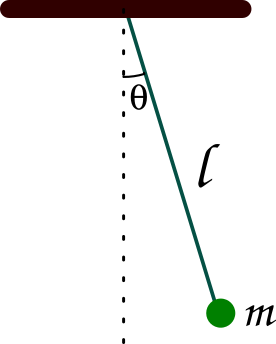
\includegraphics[width=0.3 \textwidth]{./figure1.png}
\caption{\label{fig:org673929b}pendulum with string lenth \(l\) and mass \(m\)}
\end{figure}

For understanding consequences of approximation, we took simulations by solving both equation of motion (approximated and exact). For getting equations of motion we used \textbf{Newtonian formulation} which is quite easy to work with in this type of problems, since we are working with \textbf{non conservative} system.


\subsection{Pendulum motion in presence of damping force}
\label{sec:org38c3a8a}

In real situations we have non-conservative forces affecting on system. In our system we have air resistance acting on bob. This drag force will always be proportional to it's physical shape and size. Since, we can't tell exactly drag force mathematically, We have \textbf{two often used approximations}. Firstly, there is stockes's law of drag which is linearly proportional to the velocity. Then we have Newton's drag law which is quadratically proportional to the velocity.

We will see that how this two approximation affect our system and it's simulation. We also see mathematical forms of this two but firstly, let's define this two damping coefficient.

\subsubsection{Damping by linear to the velocity approximation}
\label{sec:org6b15d0a}

Let's discuss coffiecient of linear damping. Linear to the velocity drag is also called stoke's drag. We can write equation of damping by \(F_{damping} = k_{l}v\). Where, \(k_{l}\) is damping coefficient, value of it depend on shape of object. For our spherical bob it has for of \(k_{l} = 3\pi\eta d\), where \(\eta\) is dynamic viscosity of medium and have values of \(\eta = \rho \nu\). We have \(d\) as diameter of sphere, for our purpose we are using as \(d=0.01m\). 

\subsubsection{Damping by nonlinar to the velocity approximation}
\label{sec:org68c5fbd}

We used quadratic damping approximation as nonlinear damping approximation. This is also called newton's drag and it's better approximation then linear one. As quantitatively it can work with turbulent flow with 1000 to 100000 reynolds number. Where linear approximation works reynold's number upto 1. Quadratic damping is better than linear approximation but we can't have close form solution, it is the reason we use linear damping approximation. In quadratic damping it has following form, \(F_{damping} = k_{q} v^{2}\). Here, \(k_{q} = \frac{1}{8}c_{d}\rho \pi d^{2}\), where \(c_{d}\) is drag coefficient and has value of 0.47. \(\rho\) and \(d\) are density of fluid and diameter.\cite{lubarda2021analysis}\cite{goossens2019review}


\subsection{General equation motion}
\label{sec:org97af04b}

Let's derive equation of motion for our system which can be modified as we took approximations in it. We have Figure 1 showing pendulum with unextensible string of length \(l\) with sphere of diameter \(d\) and mass \(m\). Our system is in fluid with density \(\rho\) and viscosity \(\eta\). Let's use newton's law of motion to derive equation of motion,

First of all, we compared horizontal and vertical forces.

\begin{equation}
\label{eq:org9466630}
   F_{damping}cos(\theta)-Tsin(\theta)=ma_{x}
\end{equation}
\begin{equation}
\label{eq:orgb99c293}
   F_{damping}sin(\theta)+Tcos(\theta)-mg=ma_{y}
\end{equation}

Adding equation \ref{eq:org9466630} and equation \ref{eq:orgb99c293} with multiplication by \(cos(\theta)\) and \(sin(\theta)\) respectively.

\begin{equation*}
\label{eq:org29dbf24}
F_{damping}sin^{2}(\theta)+F_{damping}cos^{2}(\theta)-mgsin(\theta)=ma_{x}cos(\theta)+ma_{y}sin(\theta)
\end{equation*}

\begin{equation*}
\label{eq:org760e1bb}
F_{damping}-mgsin(\theta)=m(asin^{2}(\theta)+acos^{2}(\theta))
\end{equation*}

\begin{equation}
\label{eq:org66f6102}
F_{damping}-mgsin(\theta)=ma
\end{equation}

From,
\begin{equation*}
\label{eq:org4b2ded3}
a = (\ddot{r}-r\dot{\theta}^{2})\hat{r} + (r \ddot{\theta}+2\dot{r}\dot{\theta})\hat{\theta}
\end{equation*}

Where,  \(r=l\) and since \(\dot{l}=0\), \(a=l\ddot{\theta}\). So, equation \ref{eq:org66f6102} becomes,

\begin{equation}
\label{eq:org9ffa3ad}
F_{damping}-mgsin(\theta)=ml\ddot{\theta}
\end{equation}

This is \textbf{exact equation of motion}. Which will be \textbf{second order non linear equation}. Finding it's exact solution is another ordeal. Let's take our approximations and cases for it.

\subsection{Approximation of equation of motion : Linear differential equation with linear damping}
\label{sec:org0c5ae05}

In class, we approximated equation \ref{eq:org9ffa3ad} as \(\theta \to 0\) as \(sin(\theta) \to \theta\). Consequently, this equation becomes very easy to solve. Also, damping force will be,

\begin{equation*}
\label{eq:orge7bf037}
F_{damping}=-k_{l}v
\end{equation*}

\begin{equation*}
\label{eq:orga31bb06}
F_{damping}=-k_{l}l\dot{\theta}
\end{equation*}

So, equation \ref{eq:org9ffa3ad} becomes,

\begin{equation}
\label{eq:org832e462}
\ddot{\theta}+\frac{k_{l}l}{m}\dot{\theta}+\frac{g}{l}\theta=0
\end{equation}

\begin{equation}
\label{eq:orgc2a99f4}
\ddot{\theta}+\Gamma\dot{\theta}+w_{0}^{2}\theta=0
\end{equation}

Where, we took \(\Gamma = \frac{k_{l}l}{m}\) and \(w_{0}^{2}\).

We can solve this linear equation \ref{eq:orgc2a99f4} by usual methods of linear differential equation. Simply taking \(\theta=e^{\lambda t}\), which gives polynomials of second order.

\begin{equation}
\label{eq:org8455fc8}
\lambda^{2}+\Gamma\lambda+w_{0}^{2}=0
\end{equation}

We can find roots of this quadratic equation.

\begin{equation}
\label{eq:org11ba213}
\lambda = \frac{-\Gamma}{2} \pm \frac{\sqrt{\Gamma^{2}-4w_{0}^{2}}}{2}
\end{equation}

\begin{equation}
\label{eq:orgf108521}
\lambda = \frac{-\Gamma}{2} \pm \sqrt{\frac{\Gamma}{2}^{2}-w_{0}^{2}}
\end{equation}

Here we getting three type of roots,

\begin{enumerate}
\item Roots where \(\frac{\Gamma}{2}=w\). this is \textbf{critical damping condition}, where we getting \(\lambda=\frac{-\Gamma}{2}\). Putting \(\lambda\) into our solutions, \(\theta = e^{\frac{-\Gamma}{2}t}\). Which suggest this will only decay with time and never overshoots from equilibrium position. Which is desired in certain condition but not for us.

\item Roots where \(\frac{\Gamma}{2}>w\). this is \textbf{overdamping condition}, where we getting \(\lambda=\frac{-\Gamma}{2}\pm\sqrt{\frac{\Gamma}{2}^{2}-w_{0}^{2}}\). So from here we get \(\theta = e^{\frac{-\Gamma}{2}t}e^{\pm\sqrt{\frac{\Gamma}{2}^{2}-w_{0}^{2}}t}\). This also have exponential term in it which will only decay with time and never overshoots from equilibrium position.

\item Roots where \(\frac{\Gamma}{2}<w\). this is \textbf{underdamping condition}, here  \(\lambda=\frac{-\Gamma}{2}\pm i\sqrt{w_{0}^{2}-\frac{\Gamma}{2}^{2}}\). \(\theta = e^{\frac{-\Gamma}{2}t}e^{\pm i \sqrt{w_{0}^{2}-\frac{\Gamma}{2}^{2}}t}\). This has complex term, which implicitly suggest that it'll overshoot and oscillate. This our topic of interest for this project.
\end{enumerate}


Without forgetting our initial system we came to we took third case as our solution.

\begin{equation*}
\label{eq:orge594baf}
\Therefore \theta = e^{\frac{-\Gamma}{2}t}e^{\pm i \sqrt{w_{0}^{2}-\frac{\Gamma}{2}^{2}}t}
\end{equation*}

Taking \(w^{2} = w_{0}^{2}-\frac{\Gamma}{2}^{2}\). And writing our solution in linear combination from above equation,

\begin{equation}
\label{eq:org292f6cb}
\theta = e^{\frac{-\Gamma}{2}t}(C_{1}e^{iwt}+C_{2}e^{-iwt})
\end{equation}

Taking real part of equation \ref{eq:org292f6cb}. Since it'll represent real motion of system. At last we get equation like this,

\begin{equation}
\label{eq:orga5d27d2}
\theta = e^{\frac{-\Gamma}{2}t}A cos(wt-\delta)
\end{equation}

Where, \(A\) and \(\delta\) can be find from initial conditions and \(w = \sqrt{w_{0}^{2}-\frac{\Gamma}{2}^{2}}\).

\subsection{Non linear equation of motion with linear damping}
\label{sec:orgeed83eb}

In equation \ref{eq:org9ffa3ad} we can write linear damping term without taking approximation as \(sin(\theta) \to \theta\),

Writing again \ref{eq:org9ffa3ad}, 
\begin{equation*}
\label{eq:org2de7a26}
F_{damping}-mgsin(\theta)=ml\ddot{\theta}
\end{equation*}

Here, putting \(F_{damping}=-k_{l}l\dot{\theta}\) will give us,

\begin{equation}
\label{eq:orgd177085}
\ddot{\theta}+\frac{k_{l}l}{m}\dot{\theta}+\frac{g}{l}sin(\theta)=0
\end{equation}

This is second order nonlinear equation we can't get it's closed form solution but we can get numerical one. Let's make it easy to use in numerical methods.

Take \(\phi = \dot{\theta}\) and \$\frac\{k\textsubscript{l}l\}\{m\}=\(\Gamma\)\$so, equation \ref{eq:orgd177085} becomes,

\begin{equation}
\label{eq:org16e2d0c}
\dot{\phi}+\Gamma\phi=-\frac{g}{l} sin(\theta)
\end{equation}

We can use numerical methods like Runge-Kutta method to solve this equation. I have given brief overview of runge kutta methods in appendix 1. For that we define \(\phi\) and \(\dot{\phi}\) as following,

\begin{equation}
\label{eq:org77ee4f6}
\phi=\dot{\theta}
\end{equation}

\begin{equation}
\label{eq:orgeef4963}
\dot{\phi}=-\Gamma\phi-\frac{g}{l} sin(\theta)
\end{equation}



\subsection{Simulations of the two equation}
\label{sec:org4ab607b}

I have done nice simulation which give hands on experience of two equation, both have very similar results when \(\theta\) is very small, again understandable as \(\theta \to 0\) we can approximate \(sin(\theta) \to \theta\). But when \(\theta\) increase slightly we have massive changes in solution with time. Let's look at \(\theta = \frac{\pi}{10}\), (here, we take viscosity of air at \((1834·38\pm0.35)\times10^{−7}\) c.g.s. units. \cite{majumdar1938coefficient})

Initially both are same as you can see in pictures (at \(t=0\)),
\begin{center}
\begin{figure}[htbp]
\centering
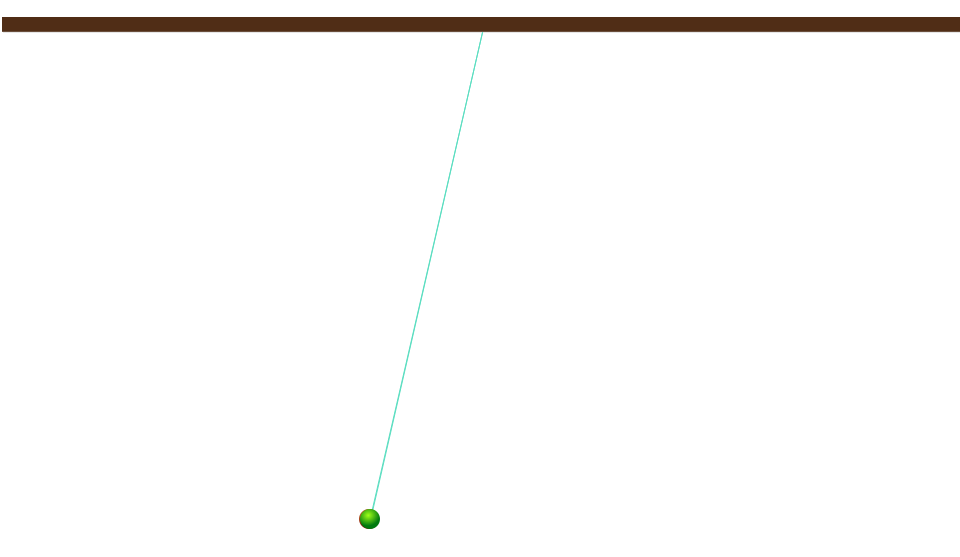
\includegraphics[width=0.8 \textwidth]{t0.png}
\caption{\label{fig:orge198a76}pendulum at \(t=0s\)}
\end{figure}
\begin{figure}[htbp]
\centering
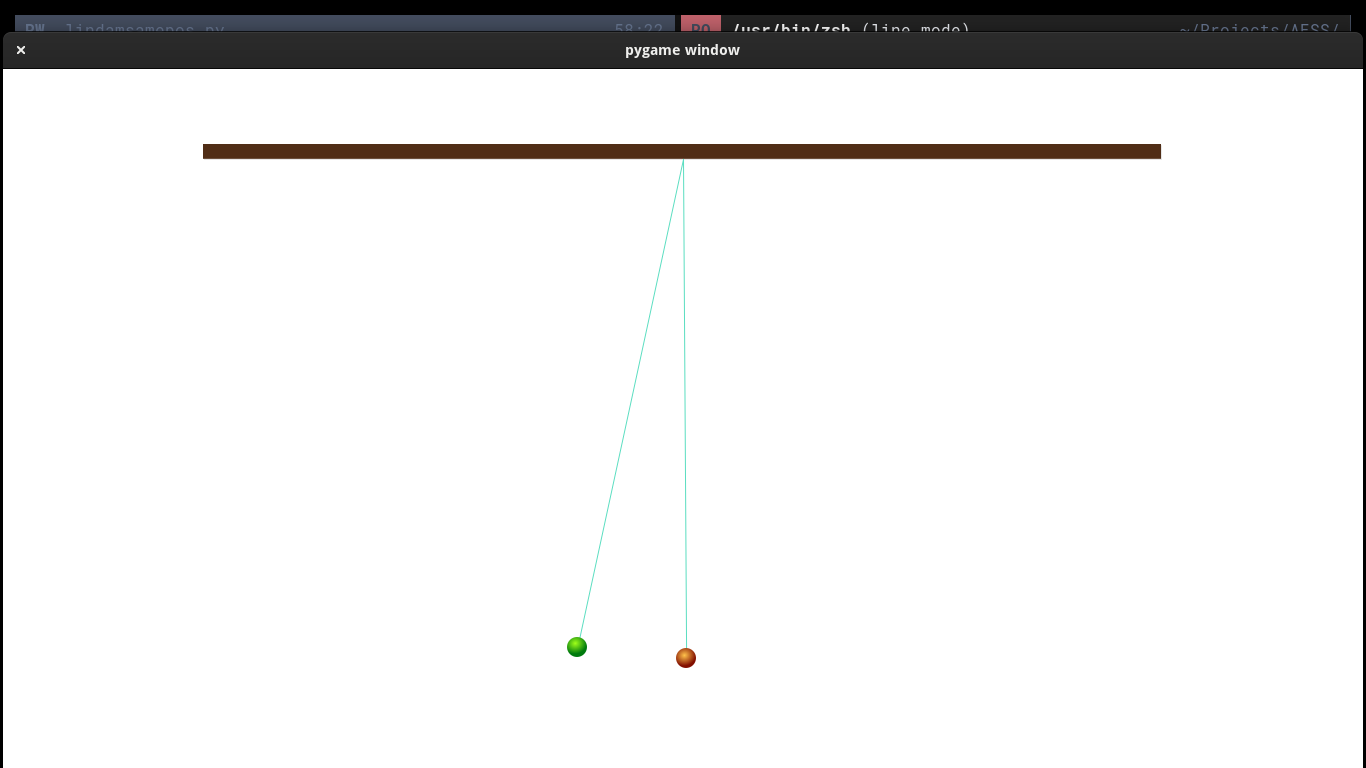
\includegraphics[width=0.8 \textwidth]{t100.png}
\caption{\label{fig:org8ff0b09}pendulum at \(t=100s\)}
\end{figure}
\end{center}



Now, as we look with increment in time we can see it deflecting slightly with it. This is picture at \(t = 100s\),















\section{appendix}
\label{sec:orgc6f06c9}
\subsection{Understanding with little simulations}
\label{sec:org7a39735}

For understaning what is we want to tell. Basically we made simulation of both the equation of motion side by side. This simulation tales that motion of both solution will be very near onto small position where \(\theta\) is quite small, but not from other. We also, try to compare with physical model \textbf{give nice view}.

Firstly exact equation of motion is nonlinear differential equation. We can't get exact solution of it. So, we just use numerical methods. We use \textbf{fourth order Runge-Kutta method}. Basically, we elaborated whole method in short down here. 

\subsubsection{Understand Runge-Kutta method}
\label{sec:org7e14d13}

In our this simulation we made use of Range Kutta fourth order method as numerical method for solving non-linear differential equation and linear differential equation with it. So, it is good idea to understand what is Range-Kutta fourth order method and how can we implement to solve present differential equations.

Runge Kutta Method is not predictor-corrector method like other numerical method (namely, modified Euler method, Adams-Bashmoth-Moulton method) for solving differential equation. It uses four different new variables and then simply addition and multiplication predict our initial value problem with good accuracy.






\subsubsection{Animations}
\label{sec:org015bda6}

Now, come animation part. Which we basically used \textbf{pygame} in \textbf{python}. We first get array of both solutions with interval of \(\frac{1}{60} second\) and give this data in position function in my \emph{main.py} file which just use convert each to the Cartesian coordinates from initial Polar coordinate. This is because \emph{pygame} screen rectangular coordinates with units in pixel of screen.

Following data, we used as constant which i defined in \emph{constant.py} file, as per close inspection you can see that we used C.G.S. units because of better visual on computer screen. Remember, we made this code for reconstruct purpose only.

My \emph{constant.py} file

\begin{lstlisting}language=Python]
  from math import sqrt

  # defining constants in C.G.S.


  width,height = 1360,720         # pygame window size in pixel units
  origin_x,origin_y = width/2,height/8 # setting up the origin O
  b = 100                              # damping coefficient
  m = 100                              # 100 grams of mass
  l = 100                              # 100 cm length
  g = 980                              # gravitation accelaraiotion in cgs

  gamma = b/m

  w0 = sqrt(g/l)                  # natural frequncy of SHM
  theta_initial = 3.141591/4      # initial theta in radian
  radius = 10                     # radius of ball in pixel
  fps = 60                        # frame per second
\end{lstlisting}

This is my \emph{main.py} file, in which i defined all functions for calculations. In which, i have Runge-Kutta method defined and solution and also phase planes defined.

\begin{lstlisting}[language=Python]
  from constants import *
  from numpy import sin, sqrt, zeros

  def f2nonlinear(theta,phi):     # we defined second auxillary equation from nonlinear term.
  return -((gamma/m)*phi*phi)-(w0*sin(theta))

  def f2linear(theta,phi):        # we defined second auxillary equation from linear term.
  return -((gamma/m)*phi*phi)-(w0*theta)

  # range-kutta method defined
  def RK4(t,theta,phi,h,K): 
  h = h/8
  for i in range(8):
  k1 = h*phi
  l1 = h*K(theta,phi)
  k2 = h*(phi+(l1*0.5))
  l2 = h*(K(theta+(k1*0.5),phi+(l1*0.5)))
  k3 = h*(phi+(l2*0.5))
  l3 = h*(K(theta+(k2*0.5),phi+(l2*0.5)))
  k4 = h*(phi+l3)
  l4 = h*(K(theta+k3,phi+l3))
  k_ = (1/6)*(k1+k4+2*(k2+k3))
  l_ = (1/6)*(l1+l4+2*(l2+l3))
  t+=h
  theta+=k_
  phi+=l_
  return  t,theta,phi

  # Solutions of linear term ---- gives array of length (Total_time*fps)
  def linear(theta_initial,Total_time,fps):
  linear_solutions = zeros([Total_time*fps])
  linear_solutions[0] = theta_initial
  phi = zeros([Total_time*fps])
  phi[0],t,time = 0,0,0
  while t-1<Total_time*fps:
  time, linear_solutions[t+1], phi[t+1] = RK4(time,linear_solutions[t],phi[t],1/fps,f2linear)
  t+=1
  return linear_solutions

  # Solutions of nonlinear term ---- gives array of length (Total_time*fps)
  def nonlinear(theta_initial,Total_time,fps):
  nonlinear_solutions = zeros([Total_time*fps])
  nonlinear_solutions[0] = theta_initial
  phi = zeros([Total_time*fps])
  phi[0],t,time = 0,0,0
  while t-1<Total_time*fps:
  time, nonlinear_solutions[t+1], phi[t+1] = RK4(time,nonlinear_solutions[t],phi[t],1/fps,f2nonlinear)
  t+=1
  return nonlinear_solutions


  # ------------(for graphs)----------
  # this describes frequncy of nonlinear term.
  def w_nonliner(theta_initial):
  T = (sqrt(l/g))*(1+(0.24*(sin(0.5*theta_initial))**2)+((9/24)*(sin(theta_initial*0.5))**4))
  return 1/T

  # phase plane definations
  def linear_phase_plane(theta,phi):
  f1 = phi
  f2 = -((gamma/m)*phi*phi)-(w0*sin(theta))
  return f1,f2

  def nonlinear_phase_plane(theta,phi):
  f1 = phi
  f2 = -((gamma/m)*phi*phi)-(w0*sin(theta))
  return f1,f2

  # ----------------------------------

\end{lstlisting}

\section{What is meaning of all this ?}
\label{sec:org7cd4f08}
\section{Appendix}
\label{sec:org9787935}

This is my simulation fi


\break
\addcontentsline{toc}{section}{References}
\bibliographystyle{plain}
\bibliography{documentaion}
\end{document}